\documentclass[11pt,a4paper]{article}

\usepackage[margin=1.75cm]{geometry}
\usepackage{graphicx}
\usepackage{amsmath}
\usepackage{booktabs}
\usepackage{caption}
\usepackage{subcaption}
\usepackage{siunitx}
\usepackage{xcolor}
\usepackage{tikz}
\usetikzlibrary{positioning,arrows.meta}
\usepackage[hidelinks]{hyperref}

\DeclareCaptionLabelFormat{boldlabel}{\textbf{#1~#2}}   % bold "Figure x" / "Table x" only
\captionsetup{labelformat=boldlabel, labelsep=colon}
\captionsetup[sub]{labelformat=parens}

% figures are read straight from the repository (compile from latex/Surrogate Model/)
\graphicspath{{../../scripts and outputs/tier_3/output/}{../../media/}}

\newcommand{\repo}{https://github.com/Shass27/curiosity-perseverance-wheel-fea}
\newcommand{\tree}{\repo/tree/main}
\newcommand{\blob}{\repo/blob/main}
\newcommand{\callout}[1]{\tikz[baseline=(c.base)]\node[circle,fill=red!80!black,text=white,font=\footnotesize\bfseries,inner sep=1.2pt,minimum size=13pt](c){#1};}   % numbered GUI marker

\title{Curiosity to Perseverance Rover Wheels:\\ Surrogate Modelling of Skin Stress and Strain}
\author{Pabitra Kumar Sahoo \and Ridam Bagul \and Sibasis Panda \and Shaswath S}
\date{}

\begin{document}
\maketitle

\begin{abstract}
\noindent The earlier failure analysis showed that the \SI{2}{mm} aluminium skin of the Curiosity wheel is driven above its fatigue limit by sharp rocks. The Perseverance wheel answered with a thicker skin and revised grousers. This report quantifies that change on the curved R250 wheel panel using 440 Ansys 2025 R1 solutions, covering five grouser features, two skin thicknesses, three grouser angles, three fillet radii and five rock-contact radii. For a sharp rock, the median peak stress falls from \SI{86}{MPa} on a Curiosity-like panel to \SI{19}{MPa} on a Perseverance-like panel. A surrogate model built from principal component analysis and Gaussian-process regression predicts the full stress and strain maps and the peak with a 95\% confidence band; on unseen geometries its median peak-stress error is 3.1\%, with 94\% band coverage. An interactive MATLAB GUI makes the model available for design exploration.
\end{abstract}

% ---------------------------------------------------------------
\section{Introduction}

The earlier failure analysis idealised a Curiosity skin segment as a flat stepped beam and showed that a sharp rock ($a \approx \SI{2}{mm}$) at \SI{400}{N} pushes the stress at the panel centre above the \SI{106}{MPa} fatigue limit of Al 7075-T7351~\cite{nasa}. For Perseverance, the wheel was redesigned with a thicker skin and a different grouser pattern. This study asks how much those changes buy, and how to search the design space between them without solving a new finite-element model for every candidate.

The study uses the real curved geometry: a \SI{45}{\degree} arc of the R250 wheel panel with its ends fixed and a \SI{300}{N} rock load on a circular patch of radius $R$ at the panel centre. Five grouser features are modelled (Figure~\ref{fig:features}). Feature~1 at $t = \SI{2}{mm}$ is treated as \emph{representative} of the Curiosity wheel and Feature~4 at $t = \SI{7.5}{mm}$ as \emph{representative} of the Perseverance redesign; neither is claimed to be the exact flight geometry. Each design point needs a new mesh and solve, so a surrogate model is trained on the solved cases to give instant predictions for any combination of inputs. All data and scripts are in the project repository~\cite{repo}.

\begin{figure}[!htb]
  \centering
  \begin{subfigure}[b]{0.32\textwidth}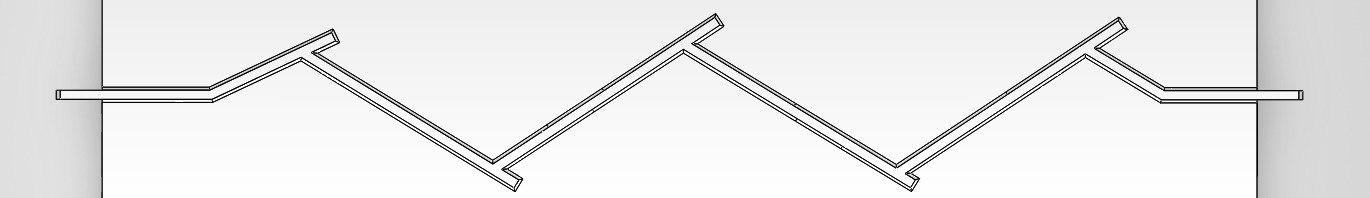
\includegraphics[width=\linewidth]{feature 1.jpeg}\caption{Feature 1 (Curiosity-like)}\end{subfigure}\hfill
  \begin{subfigure}[b]{0.32\textwidth}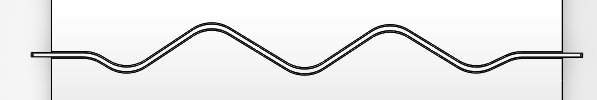
\includegraphics[width=\linewidth]{feature 2.jpeg}\caption{Feature 2}\end{subfigure}\hfill
  \begin{subfigure}[b]{0.32\textwidth}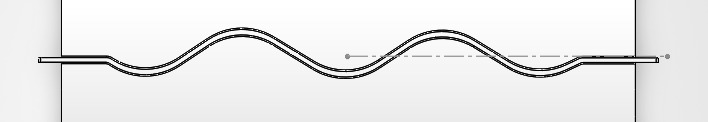
\includegraphics[width=\linewidth]{feature 3.jpeg}\caption{Feature 3}\end{subfigure}\\[6pt]
  \begin{subfigure}[b]{0.32\textwidth}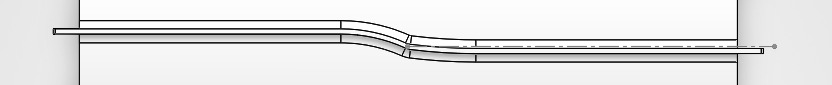
\includegraphics[width=\linewidth]{feature 4.jpeg}\caption{Feature 4 (Perseverance-like)}\end{subfigure}\hspace{0.02\textwidth}
  \begin{subfigure}[b]{0.32\textwidth}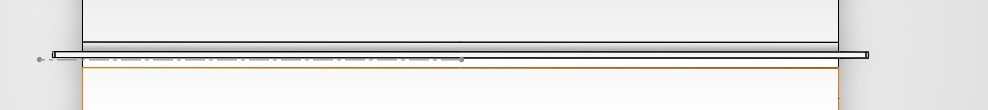
\includegraphics[width=\linewidth]{feature 5.jpeg}\caption{Feature 5}\end{subfigure}
  \caption{Plan-view grouser profiles of the five features modelled.}
  \label{fig:features}
\end{figure}

% ---------------------------------------------------------------
\section{Dataset}

Each case is set by six inputs: the feature (1--5); the skin thickness $t \in \{2, 7.5\}$\,mm; the grouser angle $s \in \{10, 12, 15\}$\,\si{\degree} (plus \SI{6}{\degree} for one Feature 4 and one Feature 5 stem); the fillet radius $r \in \{1, 3, 5\}$\,mm; the patch radius $R \in \{2, 4, 6, 8, 10\}$\,mm; and the force $F$. A \emph{stem} is one CAD geometry $(t, s, r)$ of a feature, and each stem was solved at all five values of $R$. Of the 458 solved cases, 18 Feature~5 cases with unverified load areas were excluded. The remaining 440 cases are split as 90 each for Features~1--3, 95 for Feature~4 and 75 for Feature~5. Strains exported in microstrain are converted to mm/mm. Figure~\ref{fig:sim} shows a sample run.

\begin{figure}[!htb]
  \centering
  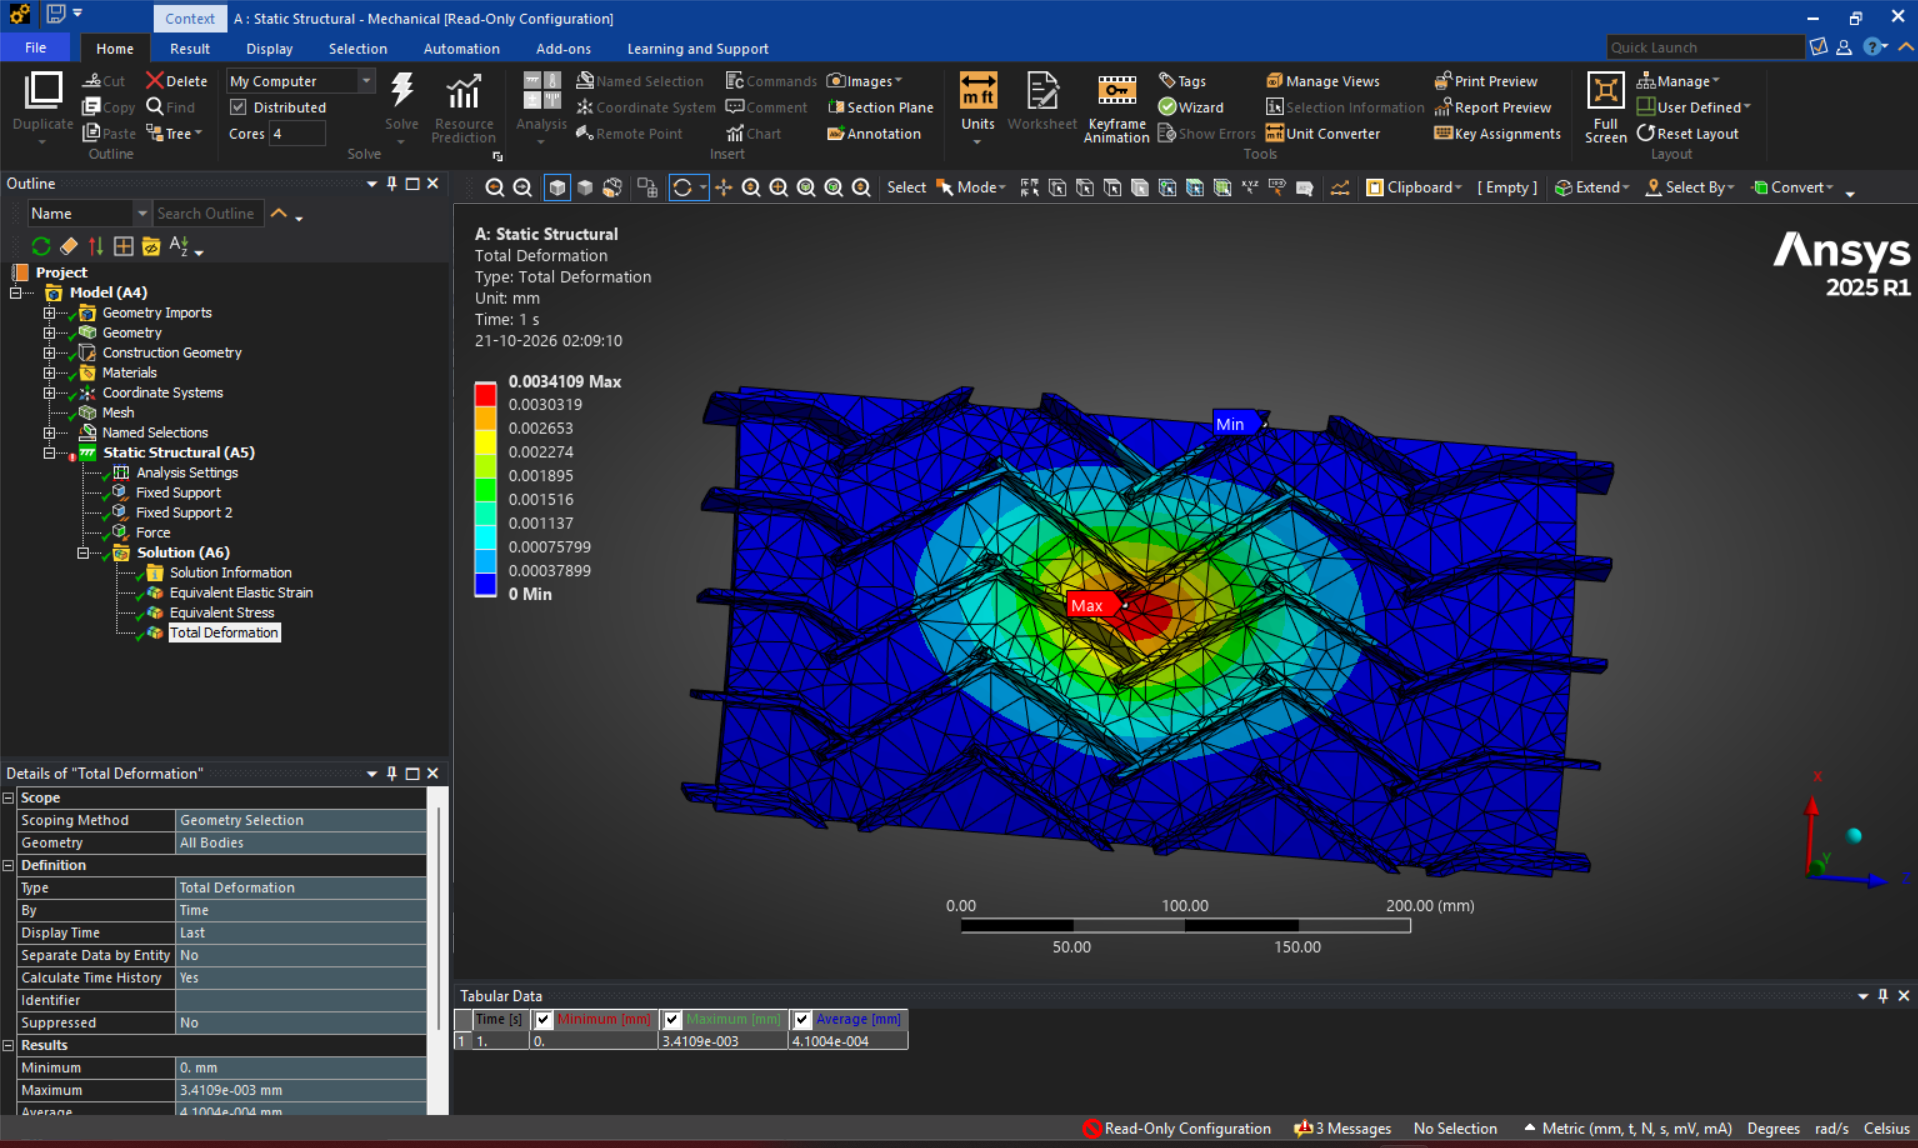
\includegraphics[width=0.85\textwidth]{deformation sim.png}
  \caption{Sample Ansys 2025 R1 run on a Curiosity wheel segment. The Equivalent Stress and Equivalent Elastic Strain results (outline, left) are the surrogate data; the total deformation contour is shown for visualisation only and is not part of this study.}
  \label{fig:sim}
\end{figure}

The nodal von Mises stress and equivalent elastic strain are exported on a different mesh for every case. To give every case the same shape, each node is mapped to the arc length $u = 250\,\text{atan2}(X, Y)$ along the R250 surface and its axial position $Z$, and binned onto a fixed grid of \SI{6}{mm} cells. This gives a $33 \times 69$ grid, or 2277 cells, covering $|u| \le \SI{98.2}{mm}$ and $|Z| \le \SI{204.5}{mm}$. Each cell keeps the largest nodal value inside it, so the grid maximum equals the nodal maximum, and empty cells copy their nearest filled neighbour. Both facts, and a stress-to-strain ratio of 55--\SI{80}{GPa}, are checked for every case in \href{\blob/scripts\%20and\%20outputs/tier_3/build_dataset.m}{\texttt{build\_dataset.m}}.

% ---------------------------------------------------------------
\section{Surrogate model architecture}
\label{sec:arch}

A whole field of 2277 values is too many outputs to regress directly, so the surrogate first compresses each field into a few shape coefficients and then learns how they depend on the inputs (Figure~\ref{fig:pipeline}). Stress and strain are modelled separately with the same structure, in \href{\blob/scripts\%20and\%20outputs/tier_3/train_surrogate.m}{\texttt{train\_surrogate.m}}.

\begin{figure}[!htb]
  \centering
  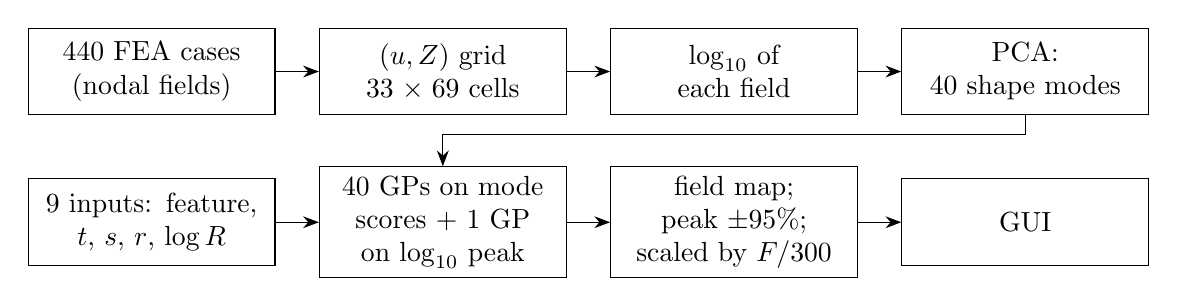
\begin{tikzpicture}[
      box/.style={draw, rectangle, align=center, minimum height=1.1cm, text width=2.9cm},
      >={Stealth[length=2mm]}, node distance=0.55cm]
    \node[box] (fea) {440 FEA cases\\(nodal fields)};
    \node[box, right=of fea] (grid) {$(u,Z)$ grid\\$33\times69$ cells};
    \node[box, right=of grid] (log) {$\log_{10}$ of\\each field};
    \node[box, right=of log] (pca) {PCA:\\40 shape modes};
    \node[box, below=0.8cm of fea] (x) {9 inputs: feature,\\$t$, $s$, $r$, $\log R$};
    \node[box, right=of x] (gps) {40 GPs on mode scores + 1 GP on $\log_{10}$ peak};
    \node[box, right=of gps] (out) {field map; peak $\pm$95\%; scaled by $F/300$};
    \node[box, right=of out] (gui) {GUI};
    \draw[->] (fea) -- (grid); \draw[->] (grid) -- (log); \draw[->] (log) -- (pca);
    \draw[->] (pca.south) |- ([yshift=4mm]gps.north) -- (gps.north);
    \draw[->] (x) -- (gps); \draw[->] (gps) -- (out); \draw[->] (out) -- (gui);
  \end{tikzpicture}
  \caption{Surrogate pipeline (one copy for stress and one for strain).}
  \label{fig:pipeline}
\end{figure}

\paragraph{Inputs.} The feature is categorical, so it is one-hot encoded as five 0/1 numbers. Thickness has only two levels, so it is a single flag. The angle $s$, fillet $r$ and $\log R$ are scaled to $[0, 1]$, giving nine inputs in all. $\log R$ is used because stress changes far more from $R = 2$ to 4 than from 8 to \SI{10}{mm}. The force is not an input: the model is linear-elastic, so every output is simply multiplied by $F/300$.

\paragraph{Log transform.} Within one panel the stress spans several orders of magnitude and is always positive. Fitting $\log_{10}$ of each cell gives every region fair weight and keeps predictions positive.

\paragraph{Principal component analysis.} The 440 log-fields are centred on their mean and decomposed into orthogonal shape modes. Each case is then described by its scores on the first modes. The target was 99.5\% of the variance, with a cap of 40 modes; the cap is reached, and the 40 modes hold 98.9\% of the variance for stress and 99.4\% for strain.

\paragraph{Gaussian-process regression.} Each mode score is learnt by its own Gaussian process (GP), fitted with MATLAB \texttt{fitrgp}~\cite{fitrgp}. A GP predicts a smooth function together with its uncertainty, which suits a small, noise-free dataset. The kernel is the automatic-relevance-determination (ARD) squared exponential, which gives each of the nine inputs its own length-scale, so the model learns how strongly each input matters. A predicted field is rebuilt by adding the predicted scores times the modes to the mean and raising the result to the power of ten.

\paragraph{Separate peak model.} The \SI{6}{mm} cells and the 40-mode truncation both smooth the sharp peaks near fillets and under the patch: a hot spot narrower than a cell appears as one bright cell, and detail beyond the 40th mode is lost. The peak value is therefore modelled directly by one more GP on $\log_{10}$ of the nodal maximum. Its predictive standard deviation gives the 95\% band reported in the GUI. In total there are 41 GPs per field and 82 for the whole surrogate.

% ---------------------------------------------------------------
\section{Training and validation}

The model is validated by five-fold cross-validation \emph{grouped by stem}. The 92 stems are randomly assigned to folds (fixed seed), and all five patch radii of a stem always fall in the same fold. Every test case is thus an unseen geometry, not just a new $R$ on a familiar one, which is the harder test. In each fold, the PCA and all GPs are refitted on the training stems only, and the held-out cases are predicted. After validation the model is refitted on all 440 cases and saved for the GUI.

Two refinements were tried and rejected. A finer \SI{5}{mm} grid lowered the stress-field $R^2$ by about 0.017 with no change in peak accuracy, and raising the cap to 160 modes improved the field $R^2$ by only about 0.003. The \SI{6}{mm}, 40-mode model was kept as the best balance of accuracy, size and GUI speed.

% ---------------------------------------------------------------
\section{Performance}

Table~\ref{tab:cv} lists the cross-validated metrics. \textbf{Field $R^2$} scores the whole predicted map against the FEA map, cell by cell, on raw (lin) or $\log_{10}$ (log) values. \textbf{Peak $R^2$} does the same for the peak value of each case only. \textbf{Median / P90 error} is the median and 90th-percentile relative error of the predicted peak. \textbf{Coverage} is the share of cases whose true peak lies inside the predicted 95\% band.

\begin{table}[!htb]
  \centering
  \caption{Five-fold stem-grouped cross-validation (\href{\blob/scripts\%20and\%20outputs/tier_3/output/cv_metrics.csv}{\texttt{cv\_metrics.csv}}).}
  \label{tab:cv}
  \begin{tabular}{llrcccccccc}
    \toprule
    & & & \multicolumn{2}{c}{Field $R^2$} & \multicolumn{2}{c}{Peak $R^2$} & \multicolumn{2}{c}{Peak error (\%)} & Coverage \\
    \cmidrule(lr){4-5}\cmidrule(lr){6-7}\cmidrule(lr){8-9}
    Field & Subset & $n$ & lin & log & lin & log & median & P90 & (\%) \\
    \midrule
    Stress & All & 440 & 0.956 & 0.979 & 0.993 & 0.996 & 3.1 & 11.3 & 93.6 \\
           & F1  &  90 & 0.949 & 0.987 & 0.992 & 0.996 & 5.0 & 11.4 & 94.4 \\
           & F2  &  90 & 0.965 & 0.992 & 0.995 & 0.995 & 3.7 & 14.0 & 90.0 \\
           & F3  &  90 & 0.959 & 0.990 & 0.990 & 0.996 & 3.9 & 12.3 & 91.1 \\
           & F4  &  95 & 0.952 & 0.953 & 0.993 & 0.993 & 2.4 & 10.5 & 93.7 \\
           & F5  &  75 & 0.949 & 0.970 & 0.995 & 0.998 & 2.5 &  6.5 & 100.0 \\
    \midrule
    Strain & All & 440 & 0.970 & 0.984 & 0.994 & 0.996 & 3.1 & 10.9 & 93.4 \\
           & F1  &  90 & 0.967 & 0.991 & 0.992 & 0.996 & 4.6 & 11.8 & 95.6 \\
           & F2  &  90 & 0.980 & 0.995 & 0.996 & 0.996 & 4.2 & 11.9 & 91.1 \\
           & F3  &  90 & 0.973 & 0.994 & 0.991 & 0.997 & 3.2 & 13.0 & 90.0 \\
           & F4  &  95 & 0.959 & 0.963 & 0.993 & 0.993 & 1.7 & 10.0 & 91.6 \\
           & F5  &  75 & 0.957 & 0.979 & 0.994 & 0.996 & 2.4 &  6.8 & 100.0 \\
    \bottomrule
  \end{tabular}
\end{table}

\begin{figure}[!htb]
  \centering
  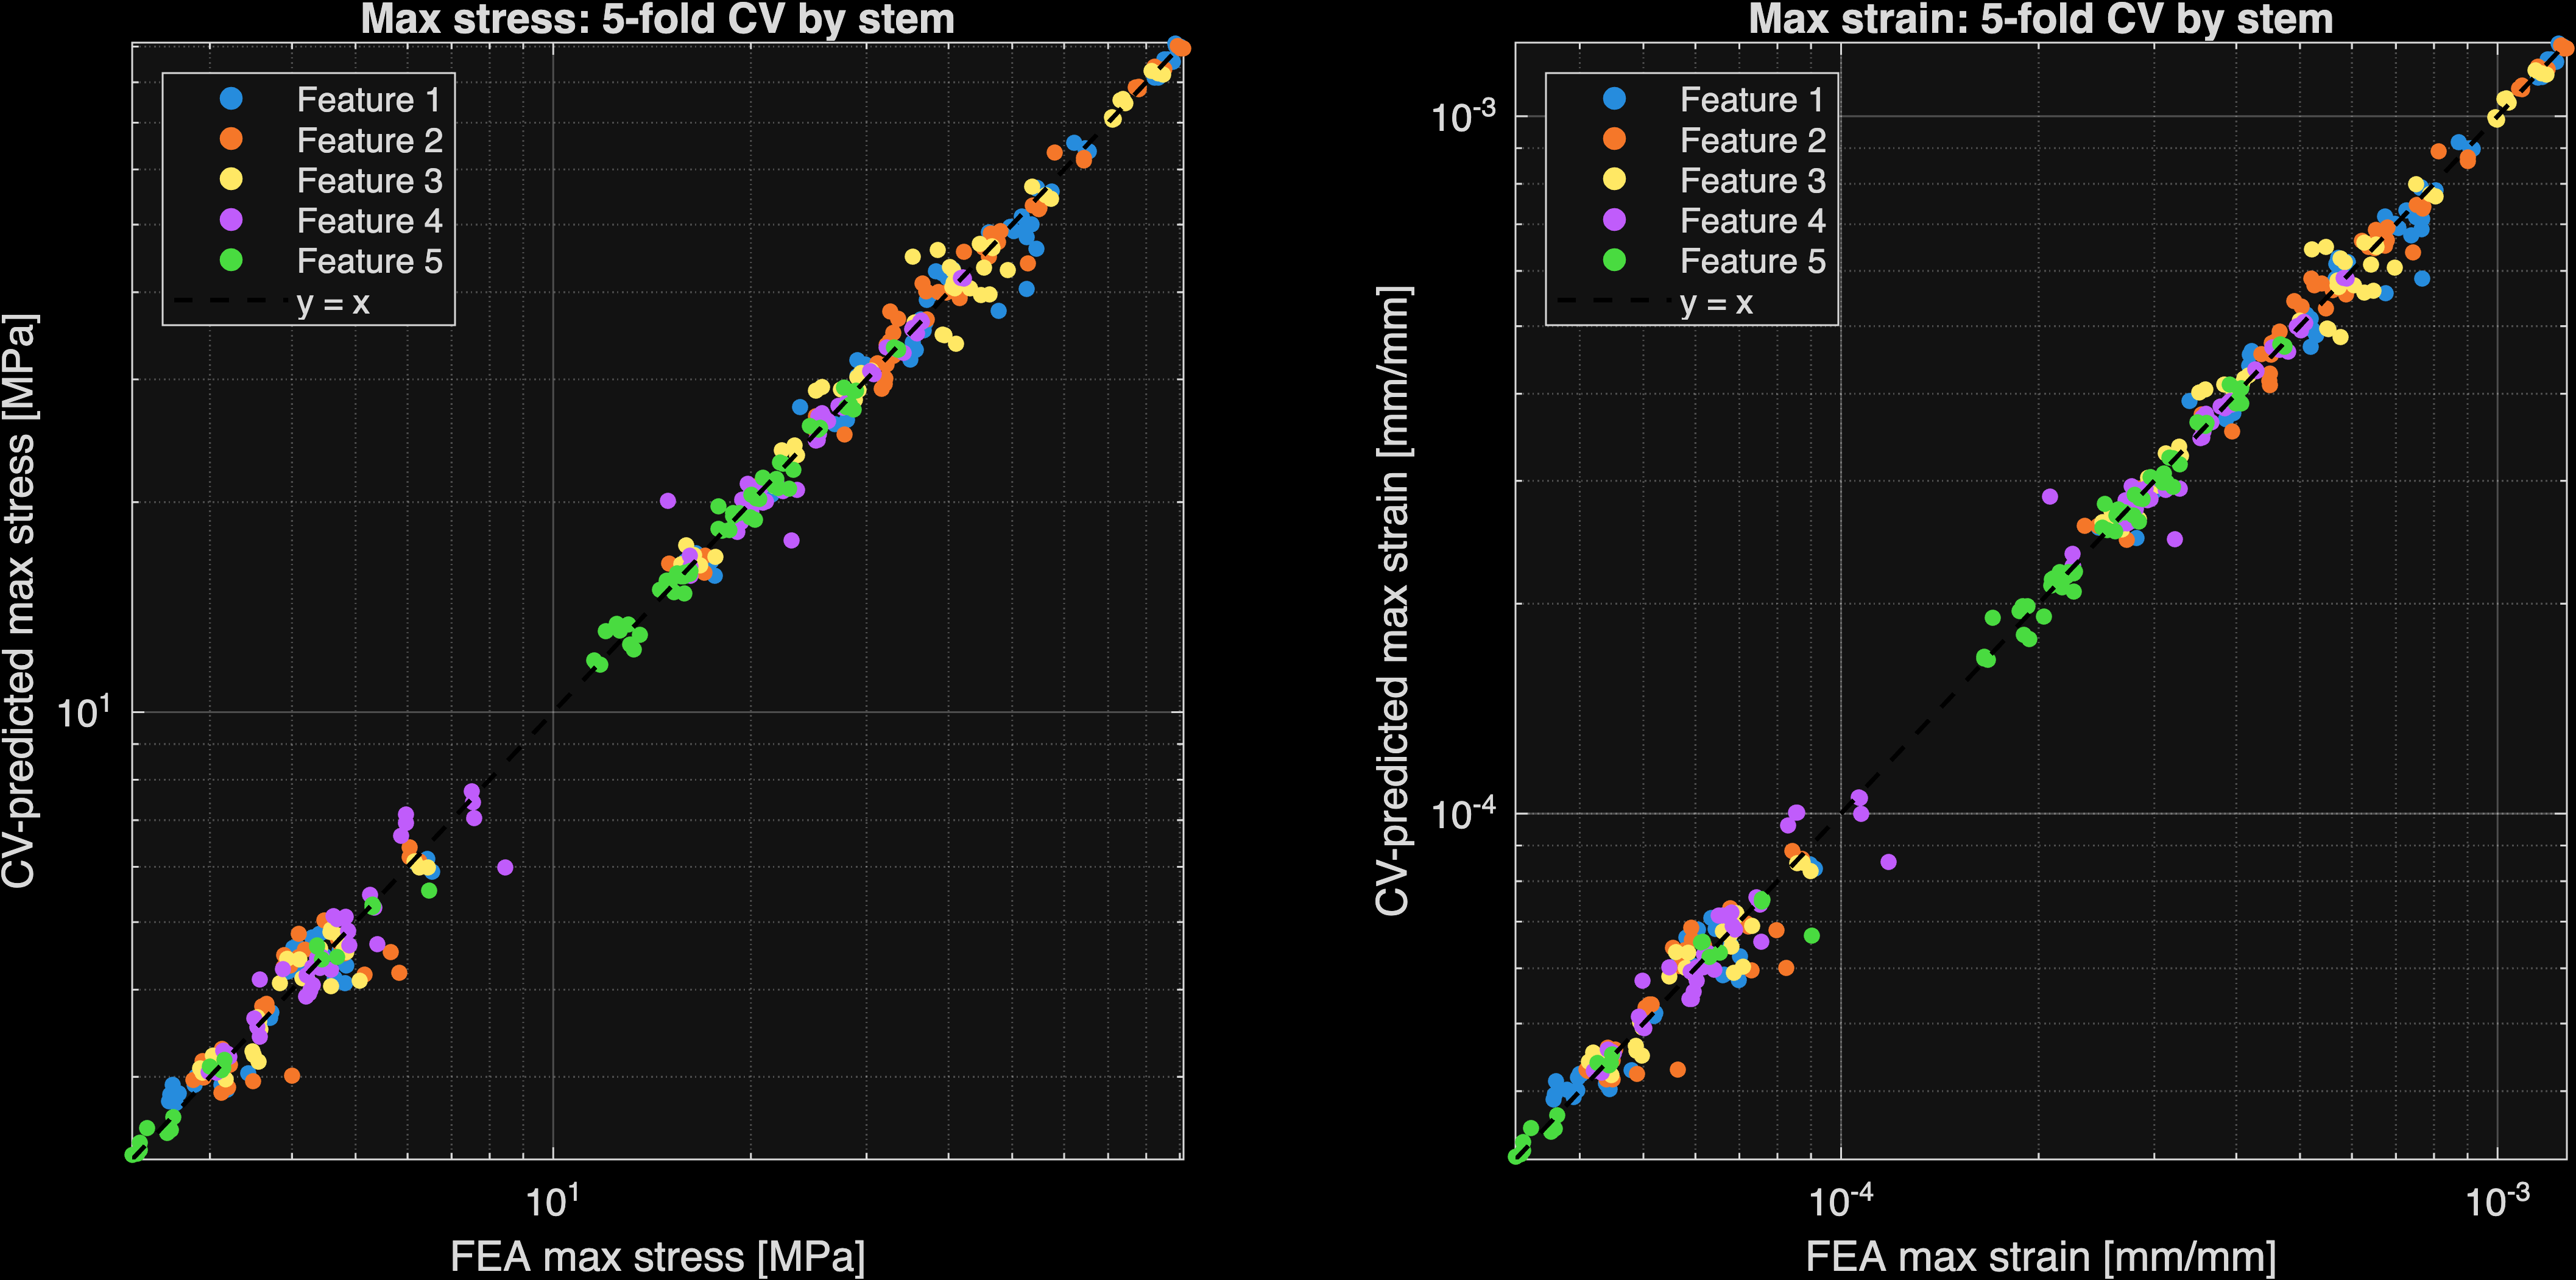
\includegraphics[width=\textwidth]{cv_parity_max.png}
  \caption{Cross-validated peak stress (left) and peak strain (right) against FEA, coloured by feature, on log axes. Points on the dashed line are exact.}
  \label{fig:parity}
\end{figure}

The surrogate predicts the peak stress with a median error of 3.1\%, and nine cases in ten are within 11.3\%. The peak $R^2$ is 0.993 on the raw values. The 95\% band contains the true peak in 93.6\% of cases, close to nominal, so it is a realistic error bar; strain behaves almost identically. The whole-map $R^2$ is lower (0.956 lin, 0.979 log) because it also scores the background and the exact location of hot spots. Feature~4 has the lowest log-field $R^2$ (0.953), consistent with its asymmetric ribs. Feature~5 has the best P90 error (6.5\%) and 100\% coverage, which suggests its bands are slightly wide. In Figure~\ref{fig:parity} the points follow the line over more than a decade; the largest scatter is in the 3--\SI{8}{MPa} cluster of stiff \SI{7.5}{mm} panels, where absolute errors are small.

% ---------------------------------------------------------------
\section{Curiosity to Perseverance: design study}

Table~\ref{tab:design} gives the median FEA peak stress for each feature, thickness and patch radius at \SI{300}{N}, taken over the grouser angles and fillet radii.

\begin{table}[!htb]
  \centering
  \caption{Median FEA peak von Mises stress (MPa) at \SI{300}{N} over all $s$ and $r$. Bold: Curiosity-like (F1, \SI{2}{mm}) and Perseverance-like (F4, \SI{7.5}{mm}).}
  \label{tab:design}
  \begin{tabular}{l rrrrr rrrrr}
    \toprule
    & \multicolumn{5}{c}{$t = \SI{2}{mm}$, $R$ (mm)} & \multicolumn{5}{c}{$t = \SI{7.5}{mm}$, $R$ (mm)} \\
    \cmidrule(lr){2-6}\cmidrule(lr){7-11}
    Feature & 2 & 4 & 6 & 8 & 10 & 2 & 4 & 6 & 8 & 10 \\
    \midrule
    F1 & \textbf{86.2} & \textbf{54.6} & \textbf{40.4} & \textbf{37.3} & \textbf{29.1} & 17.4 & 4.5 & 3.7 & 3.1 & 2.7 \\
    F2 & 84.1 & 54.9 & 41.0 & 33.5 & 32.0 & 17.0 & 4.8 & 3.7 & 3.2 & 3.2 \\
    F3 & 73.7 & 46.6 & 35.5 & 39.2 & 25.7 & 16.7 & 4.8 & 3.6 & 3.1 & 3.5 \\
    F4 & 33.3 & 26.1 & 28.0 & 25.5 & 25.3 & \textbf{19.2} & \textbf{6.0} & \textbf{4.8} & \textbf{4.4} & \textbf{4.0} \\
    F5 & 20.4 & 21.9 & 18.8 & 19.9 & 18.1 & 13.2 & 5.0 & 3.1 & 2.6 & 2.3 \\
    \bottomrule
  \end{tabular}
\end{table}

Under a sharp rock ($R = \SI{2}{mm}$), the Curiosity-like panel reaches \SI{86}{MPa}. Scaled to the \SI{400}{N} design load of the earlier failure analysis, this is about \SI{115}{MPa}, above the \SI{106}{MPa} fatigue limit, which agrees with that study's finding. The two Perseverance changes act in sequence. At \SI{2}{mm}, changing the grouser pattern from Feature~1 to Feature~4 alone more than halves the sharp-rock peak (86 to \SI{33}{MPa}), because the ribs share the load. Increasing the skin to \SI{7.5}{mm} then lowers it to \SI{19}{MPa}, about 4.5 times below Curiosity, and below \SI{6}{MPa} for blunter rocks. Every \SI{7.5}{mm} design stays far below the fatigue limit, even at \SI{400}{N}.

The FEA covers only these grid points. The surrogate fills the space between them (any $s$ in 10--\SI{15}{\degree}, $r$ in 1--\SI{5}{mm}, $R$ in 2--\SI{10}{mm} and any force) instantly and with a confidence band, so a designer can search for the design that keeps the peak below a chosen margin for a given rock and load without re-meshing. Only stress is assessed here; mass is outside this study.

% ---------------------------------------------------------------
\section{Interactive GUI}

The GUI, \href{\blob/scripts\%20and\%20outputs/tier_3/tier3_gui.m}{\texttt{tier3\_gui.m}}, loads the trained model and updates every output when an input changes (Figure~\ref{fig:gui}). Its elements are listed in Table~\ref{tab:gui}.

\begin{figure}[!htb]
  \centering
  \begin{tikzpicture}
    \node[anchor=south west, inner sep=0] (img) {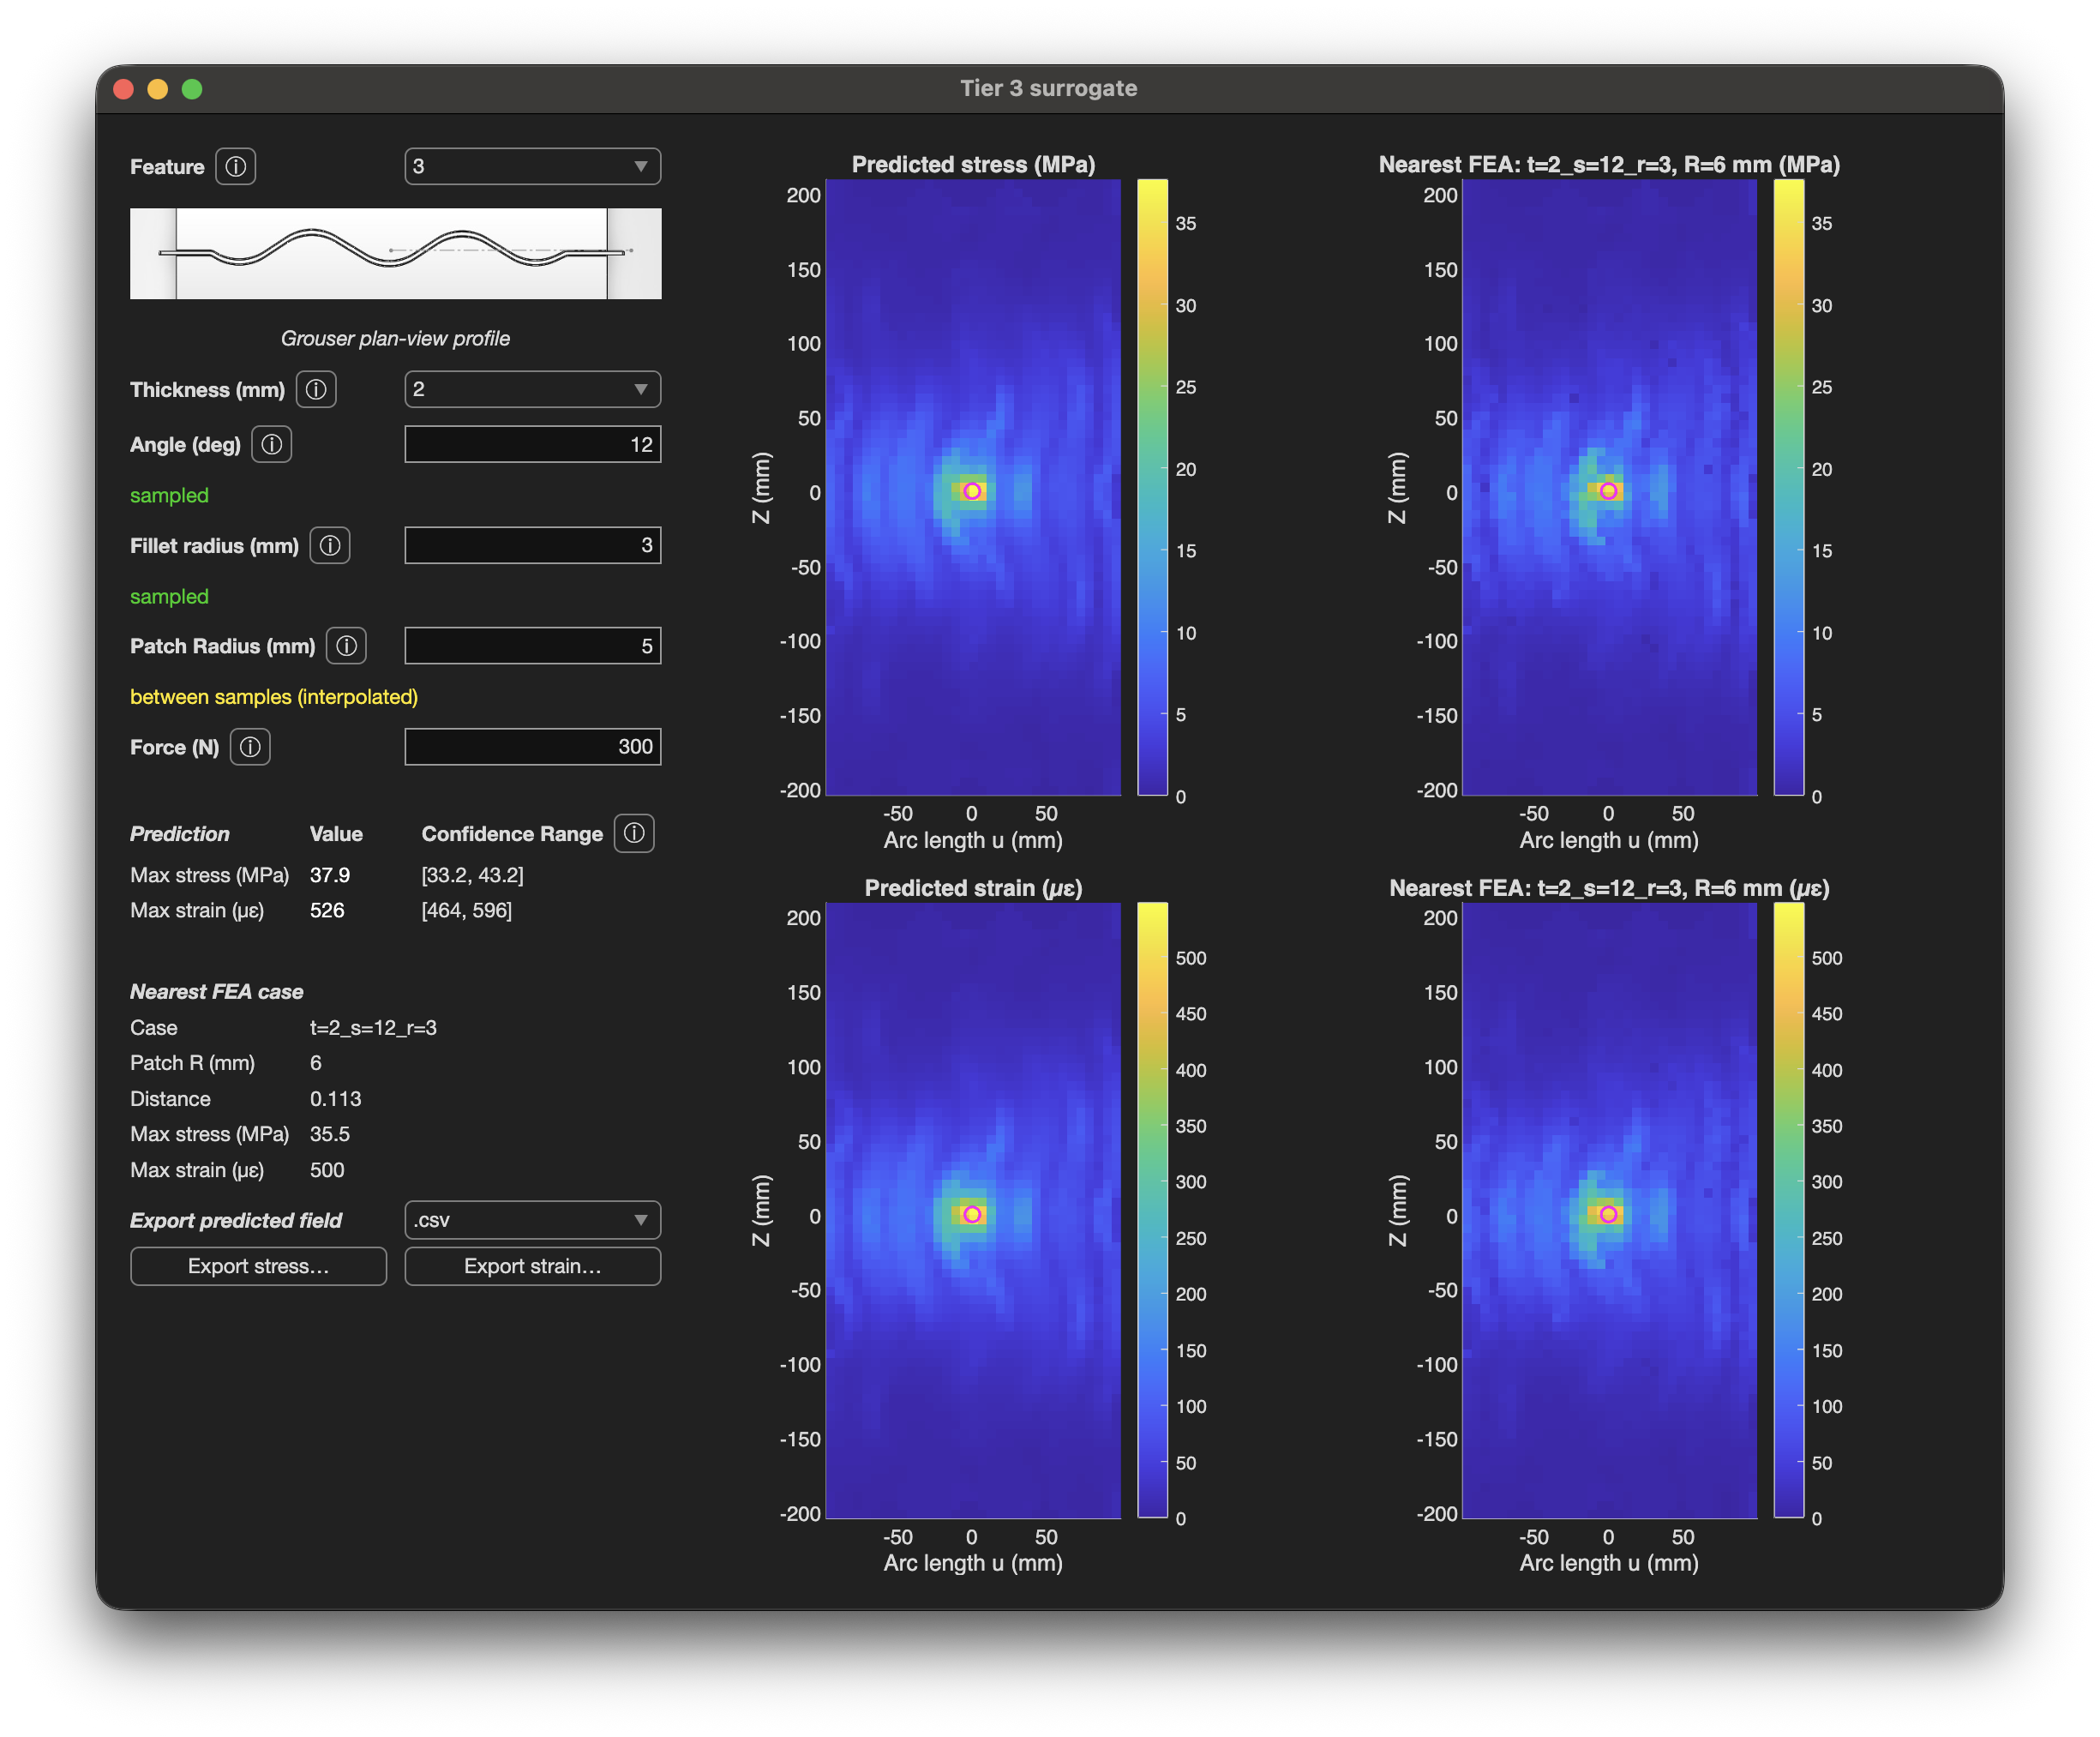
\includegraphics[width=0.9\textwidth]{Surrogate GUI.png}};
    \begin{scope}[x={(img.south east)}, y={(img.north west)}, every node/.style={circle, fill=red!80!black, text=white, font=\small\bfseries, inner sep=1.2pt, minimum size=16pt}]
      \node at (0.030, 0.904) {1};
      \node at (0.030, 0.776) {2};
      \node at (0.030, 0.599) {3};
      \node at (0.030, 0.521) {4};
      \node at (0.030, 0.429) {5};
      \node at (0.030, 0.297) {6};
      \node at (0.365, 0.906) {7};
      \node at (0.620, 0.906) {8};
    \end{scope}
  \end{tikzpicture}
  \caption{Surrogate model GUI: Feature~3, $t = \SI{2}{mm}$, $s = \SI{12}{\degree}$, $r = \SI{3}{mm}$, $R = \SI{5}{mm}$, \SI{300}{N}. Numbers refer to Table~\ref{tab:gui}.}
  \label{fig:gui}
\end{figure}

\begin{table}[!htb]
  \centering
  \small
  \caption{GUI elements.}
  \label{tab:gui}
  \begin{tabular}{c p{3.0cm} p{12.5cm}}
    \toprule
    & Element & Function \\
    \midrule
    \callout{1} & Feature selector & Feature 1--5; the grouser profile image updates with it. \\
    \callout{2} & Geometry and force inputs & $t$ (2 or \SI{7.5}{mm}), $s$, $r$, $R$ and $F$. Each \textcircled{\scriptsize i} pop-up lists the modelled values and valid range. \\
    \callout{3} & Input status & Green: simulated value; yellow: interpolated; red: outside the sampled range. Extra notes flag blended or sparsely sampled $s$ (Section~\ref{sec:limits}). \\
    \callout{4} & Prediction table & Peak stress (MPa) and strain (\si{\micro\varepsilon}) with their 95\% ranges. Red warnings above the \SI{106}{MPa} fatigue limit, 8\% failure strain and \SI{435}{MPa} yield (linear model invalid). \\
    \callout{5} & Nearest FEA case & Closest solved case of the same feature and $t$ (normalised distance in $s$, $r$, $\log R$), with its peaks scaled to $F$. \\
    \callout{6} & Export & Saves the predicted map as .xls/.csv/.txt/.xlsx/.mat in the Ansys export layout, plus a \texttt{\_summary.xls}. \\
    \callout{7} & Predicted maps & Stress and strain on $(u, Z)$; magenta circle = load patch, white contour = \SI{106}{MPa}. \\
    \callout{8} & Nearest FEA maps & FEA fields of case 5 on the same colour scale as 7, for a visual check. \\
    \bottomrule
  \end{tabular}
\end{table}

In the example shown, $R = \SI{5}{mm}$ lies between two simulated radii, so it is flagged yellow. The surrogate predicts a peak of \SI{37.9}{MPa} with a band of [33.2, 43.2]\,MPa. The nearest solved case (\texttt{t=2\_s=12\_r=3}, $R = \SI{6}{mm}$) gives \SI{35.5}{MPa}, and its field has the same shape and extent.

% ---------------------------------------------------------------
\section{Limitations}
\label{sec:limits}

\paragraph{Grid resolution and mode count.} The predicted maps are \SI{6}{mm} cell maxima reconstructed from 40 modes (Section~\ref{sec:arch}), so they show the stress distribution rather than the exact local value at a fillet; the peak value should be read from the prediction table.

\paragraph{Discrete inputs and extrapolation.} Feature and thickness are categories: the model cannot predict a new grouser profile or a thickness between 2 and \SI{7.5}{mm}. Between $s = 10$ and \SI{12}{\degree} the model blends a 5-grouser and a 3-grouser layout, so the result is not a real design, and $s < \SI{10}{\degree}$ rests on a single stem. Outside the sampled ranges the GPs revert to the mean and are unreliable; the GUI flags these inputs in red. Finally, the 18 unverified Feature~5 cases are excluded, and force scaling holds only below yield.

% ---------------------------------------------------------------
\section{Conclusions}

Both Perseverance changes reduce the skin stress, in different ways. The ribbed grouser pattern of Feature~4 roughly halves the sharp-rock peak on a \SI{2}{mm} skin by sharing the load, and the thicker skin then removes most of what remains, closing the fatigue problem found in the earlier failure analysis. The surrogate model reproduces the FEA closely enough to replace it for screening, and its 95\% band is an honest error bar. Its natural next use is optimisation: finding, for a given rock size and load, the thinnest skin or the grouser angle and fillet that keep the peak below the fatigue limit, with the nearest FEA case shown alongside as a check.

% ---------------------------------------------------------------
\section*{Repository resources}
\begin{itemize}\setlength\itemsep{0pt}
  \item Dataset builder: \href{\blob/scripts\%20and\%20outputs/tier_3/build_dataset.m}{\texttt{scripts and outputs/tier\_3/build\_dataset.m}}
  \item Surrogate training and validation: \href{\blob/scripts\%20and\%20outputs/tier_3/train_surrogate.m}{\texttt{scripts and outputs/tier\_3/train\_surrogate.m}}
  \item GUI: \href{\blob/scripts\%20and\%20outputs/tier_3/tier3_gui.m}{\texttt{scripts and outputs/tier\_3/tier3\_gui.m}}
  \item Trained model, metrics and figures (with README): \href{\tree/scripts\%20and\%20outputs/tier_3/output}{\texttt{scripts and outputs/tier\_3/output}}
  \item FEA results: \href{\tree/Simulation\%20results}{\texttt{Simulation results}}
  \item Review of the excluded Feature~5 cases: \href{\blob/Simulation\%20results/NOTE.md}{\texttt{Simulation results/NOTE.md}}
  \item Images used in this report: \href{\tree/media}{\texttt{media}}
\end{itemize}

\begin{thebibliography}{9}
  \bibitem{nasa} NASA Jet Propulsion Laboratory, Mars Science Laboratory (Curiosity) and Mars 2020 (Perseverance) mission reports. \url{https://mars.nasa.gov/}
  \bibitem{fitrgp} The MathWorks, \emph{Statistics and Machine Learning Toolbox User's Guide}: \texttt{fitrgp}, Gaussian process regression.
  \bibitem{repo} Project repository, \href{\repo}{\texttt{github.com/Shass27/curiosity-perseverance-wheel-fea}}
\end{thebibliography}

\end{document}
